\documentclass[t]{beamer}

\usepackage[english]{babel}

\usepackage{float}
%\floatstyle{boxed}
%\restylefloat{figure}
\usepackage{times}
%\usepackage[T1]{fontenc}
\usepackage{graphicx}
\usepackage{hyperref}
\usepackage{listings}
\usepackage[utf8]{inputenc}
\usepackage{graphicx}
%% \usepackage{pgf,tikz}
%% \usepackage{pgfplots}
%% \usetikzlibrary{shapes,arrows,snakes,automata,backgrounds,petri,calc,trees}
%% \usetikzlibrary{matrix, positioning, fit}
%% \usepackage{smartdiagram}
%% \usepackage{mathtools}
\usepackage{ulem}


%\setbeameroption{show only notes}

\def\PresTitle{Greybeard's Guide to *NIX}
\font\footnoteFont=phvr7t at 8pt
\font\footnoteRefFont=phvro7t at 8pt
\font\thFont=phvb7t at 12pt
\newfont{\codeFont}{cmtt10 scaled 800}
\setbeamerfont{verbatim}{size={\fontsize{8pt}{10pt}}}
\mode<presentation>
{
  \usetheme{Madrid}
  \setbeamercovered{transparent}
  \usecolortheme{orchid}
}


\title[\PresTitle]{\PresTitle}
\subtitle{or, how I learned to love the command line}

\author[Steve Roggenkamp] % (optional, use only with lots of authors)
{Steve Roggenkamp\\
}

\date[13 Sep 2017] % (optional)
{13 Sep 2017 \\
  \bigskip
  \bigskip
  \bigskip
  
\includegraphics[scale=0.4]{images/cc-4_0.png}
 }

\institute[]{
 Institute for Biomedical Informatics\\
  University of Kentucky\\
  \href{mailto:steve.roggenkamp@uky.edu}{\nolinkurl{steve.roggenkamp@uky.edu}}\\
  \href{https://github.com/roggenkamps/GreybeardsGuide}{\nolinkurl{https://github.com/roggenkamps/GreybeardsGuide}}
}

\subject{\PresTitle}

\begin{document}

\frame{\titlepage}

% \begin{frame}{}
%  \begin{itemize}
%  \item Why learn to use the command line?
%  \item Six things to know
%  \end{itemize}
% \end{frame}

\begin{frame}{Why???}
  The command line is Ancient and Decrepit? Why waste time on it?
  \pause
  \begin{itemize}
  \item Systems administration
  \pause
  \item Resource constrained systems
    \begin{itemize}
    \item Embedded systems
      \pause
    \item High performance systems
    \end{itemize}
  \pause
  \item It can do a lot for you
  \end{itemize}
  \note{}
\end{frame}

\begin{frame}{What we're going to cover}
  \begin{itemize}
  \item Six essential concepts to efficiently use command line:
    \pause
    \begin{itemize}
    \item Command shell
    \pause
    \item Pipes to connect commands
    \pause
    \item Man pages for documentation
    \pause
    \item Regular expressions for text processing
    \pause
    \item \texttt{find} to query file systems
    \pause
    \item Command substitution
    \end{itemize}
    \pause
  \item Solve a practical problem with just a line or two of code
  \end{itemize}
  \note{}
\end{frame}


\begin{frame}{The Shell, a must have}
  \begin{itemize}
  \item Parses your input and executes commands, think REPL
    \pause
    \item Provides an environment in which you work
    \pause
    \item Provides a scripting programming language to automate tasks
  \end{itemize}
\end{frame}

\begin{frame}{Shells - If you don't like one, try another}
  \begin{itemize}
  \item \texttt{ash}, \texttt{bash}, \texttt{dash}
    \pause
  \item Bourne shell, Korn shell, PD Korn,  Bourne-again shell
    \pause
  \item \texttt{csh}, \texttt{tcsh}, \texttt{zsh}
    \pause
  \item Busybox (which normally uses \texttt{ash})
    \pause
  \item Each provides unique set of capabilities
    \pause
  \item Today's talk focuses on Bourne-again shell, aka, \texttt{bash}
    \begin{itemize}
    \item Default shell for most Linux and Mac OSX
      \item Available for most *NIX system
    \end{itemize}
  \end{itemize}
  \note{}
\end{frame}

\begin{frame}{Starting a shell}
  \begin{itemize}
  \item Start a terminal in a GUI environment
  \item Remotely execute a shell via \texttt{ssh}
  \item Log into a system console
  \end{itemize}
  \note{}
\end{frame}

\begin{frame}{Sample session start}
  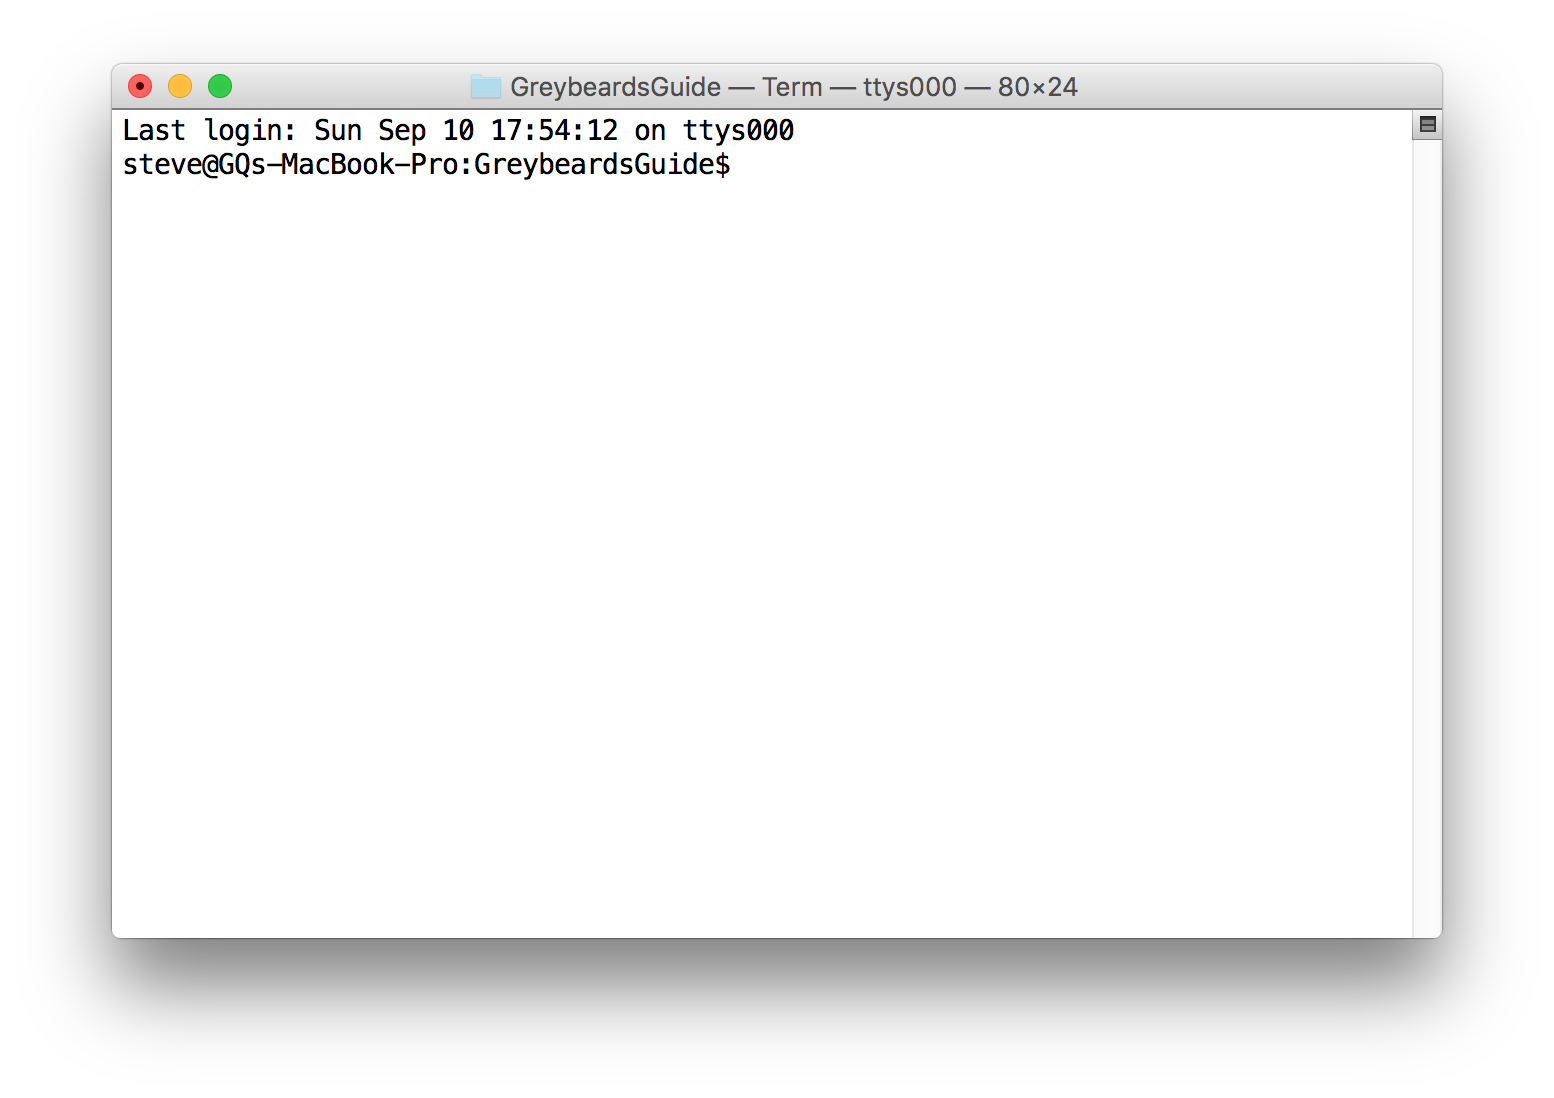
\includegraphics[width=10cm,scale=0.4]{images/newtty-1.png}

  Now what?? Coder's Block!!!
  \note{}
\end{frame}

\begin{frame}{Session - list current directory}
  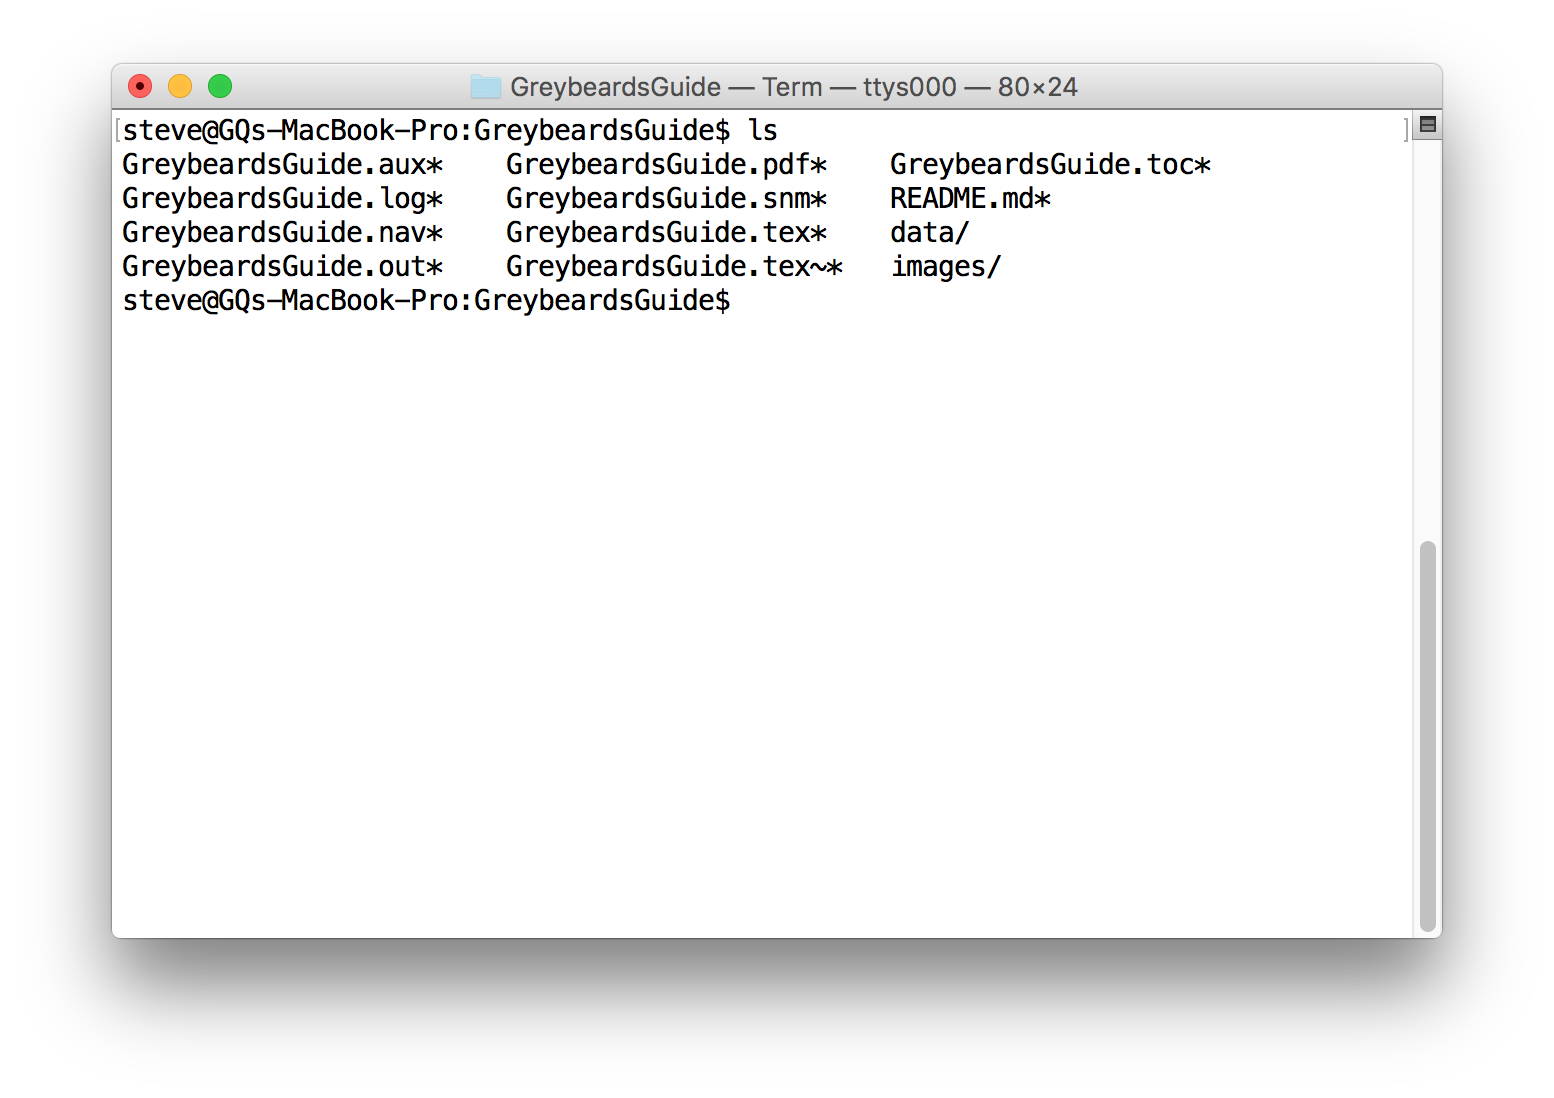
\includegraphics[width=10cm,scale=0.4]{images/newtty-2.png}

  \texttt{ls} lists the contents of a directory
  \note{}
\end{frame}

\begin{frame}{Shell - file redirection}
  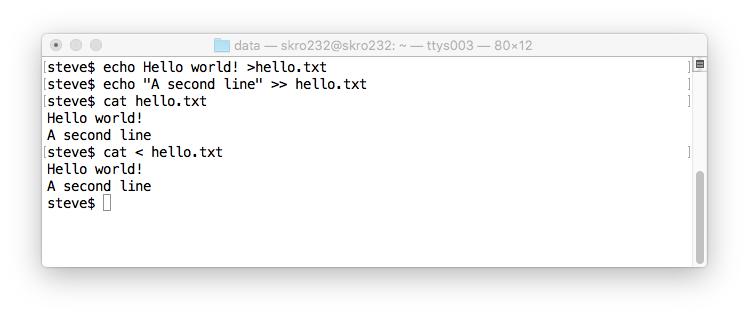
\includegraphics[width=12cm,scale=0.4]{images/file-redir.png}
  \begin{itemize}
  \item \texttt{>} redirects a program's standard output to a file
  \item \texttt{>>} appends a program's standard output to a file
  \item \texttt{<} redirects a file to a program's standard input 
  \end{itemize}
  \note{
%%        echo Hello world! > hello.txt
%%        echo ``A second line'' >> hello.txt
%%        ls -l >ls.out
%%        cat < hello.txt
%%        cat *
%%        file *
%%        echo ''ls -l'' >>cmd.txt
%%        . cmd.txt
%%        echo ``#!/bin/bash'' >cmd1.txt
%%        echo ''ls -al'' >>cmd1.txt
%%        cat >cmd2.txt <<EOF
%%        #!/bin/bash
%%        ls -al *.txt
%%        EOF
       }
\end{frame}

\begin{frame}{Shell - executing scripts}
  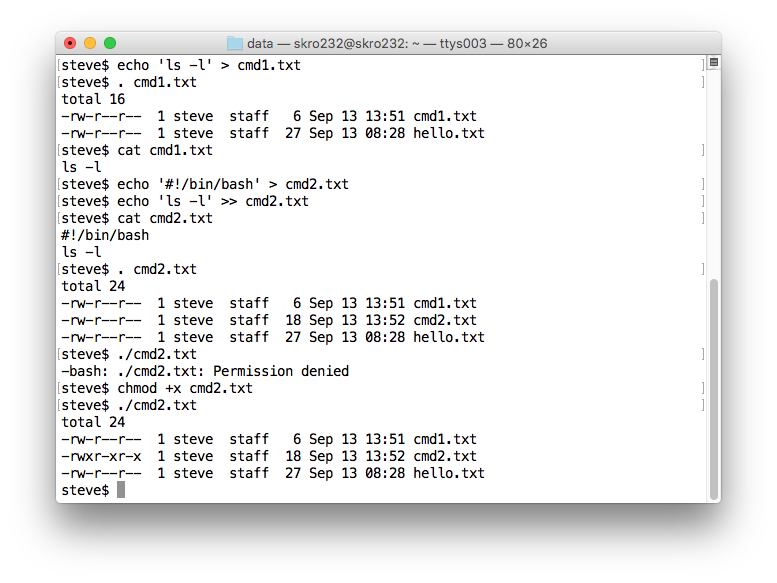
\includegraphics[width=10cm,scale=0.4]{images/scripting.png}
%  \begin{itemize}
%  \item 
%  \end{itemize}
  \note{
%%        . cmd.txt
%%        source cmd.txt
%%        chmod +x cmd[12].txt
%%        ./cmd1.txt
%%        file *
%%        ./cmd2.txt
}
\end{frame}

\begin{frame}{Shell - filename patterns}
  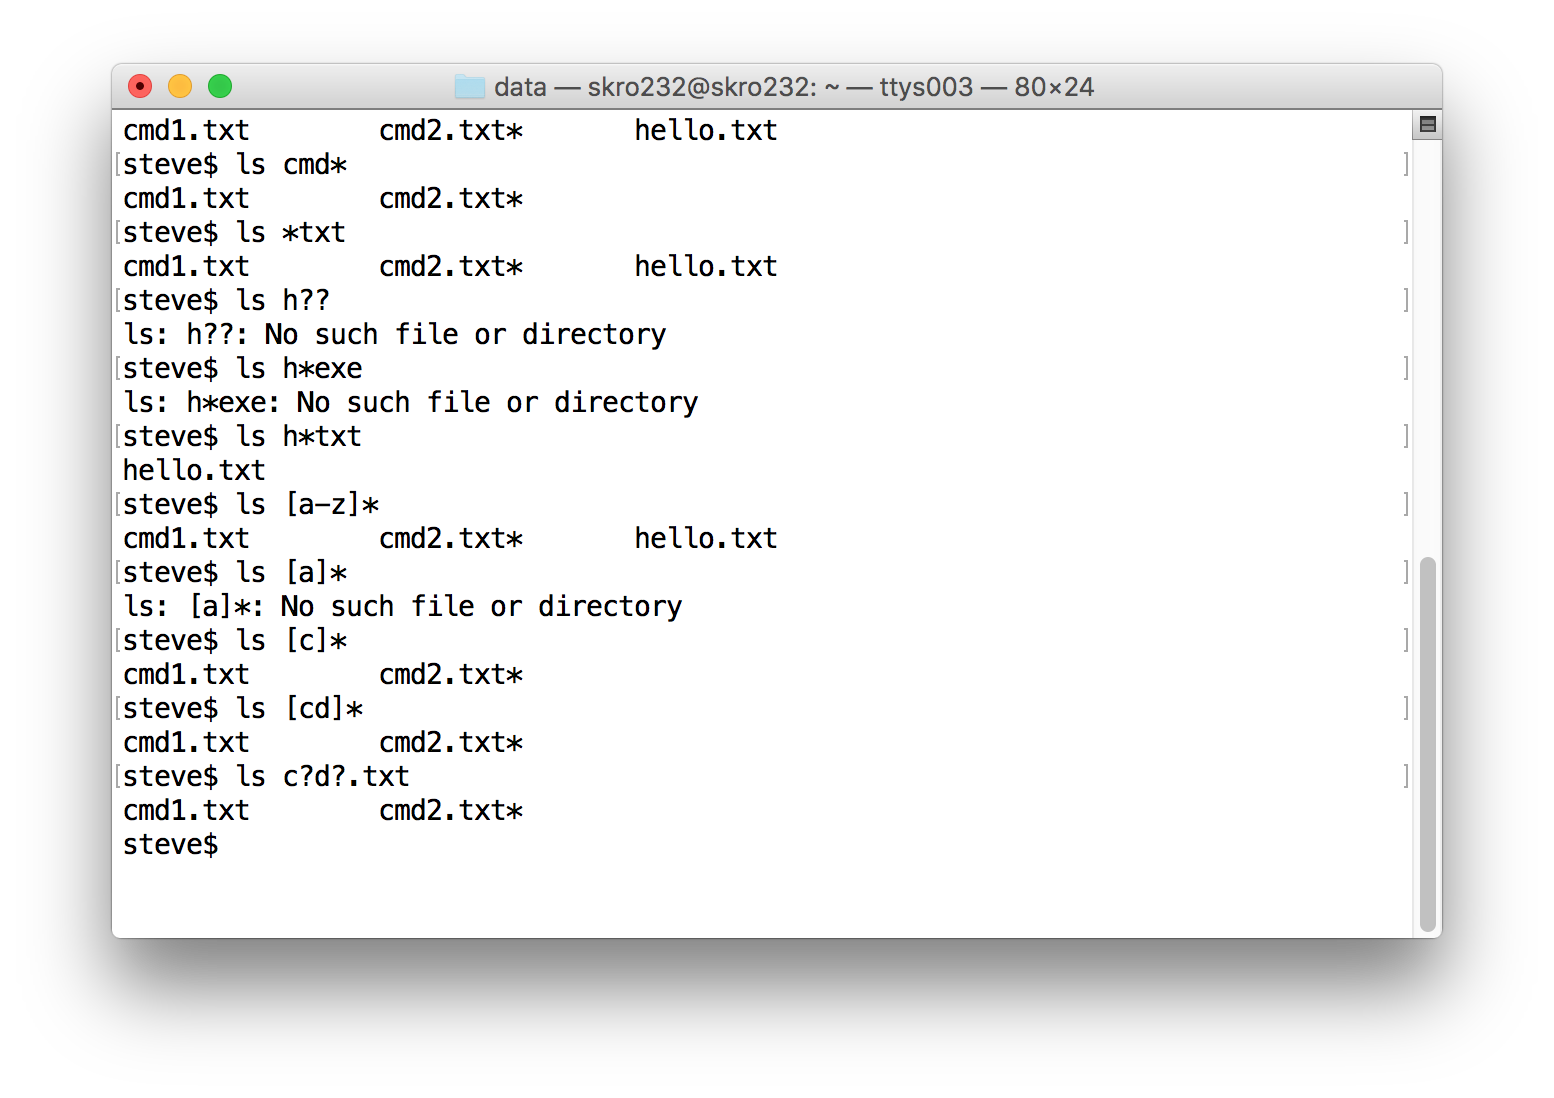
\includegraphics[width=10cm,scale=0.4]{images/filepat.png}
  \begin{itemize}
  \item *NIX does not respect ``filename extensions''
  \item 'cmd.txt' matches a file named 'cmd.txt'
  \item ? matches a single character
  \item * matches any numbers of characters
  \end{itemize}
  \note{}
\end{frame}

\begin{frame}{Shell - filename patterns, cont.}
  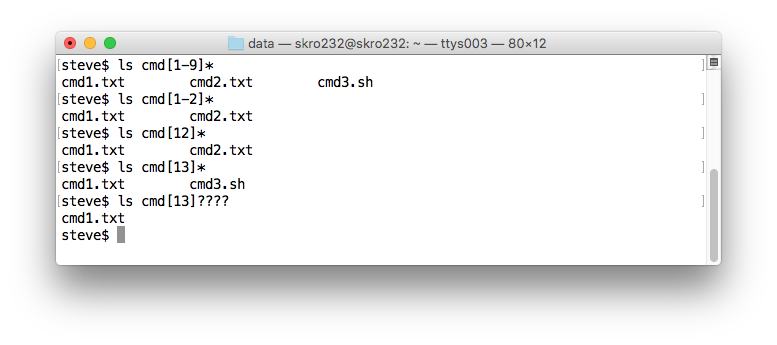
\includegraphics[width=10cm,scale=0.4]{images/filepat-1.png}
  \begin{itemize}
  \item \lbrack xy\rbrack matches characters 'x' and 'y'
  \item \lbrack x-z\rbrack matches characters between 'x' and 'z' inclusive
  \end{itemize}
  \note{}
\end{frame}

\begin{frame}{Pipes - Composing programs}
  \begin{itemize}
  \item Pipes feed the output from a program to the input of another program
  \item Allow us to string programs together for ``one-of'' programs
  \item Very efficient 
    \begin{itemize}
    \item Creates one process per program
    \item File buffer between programs
    \item Signals and scheduler coordinate writing and reading data
      between programs - no extra files needed
    \end{itemize}
  \end{itemize}
  \note{}
\end{frame}

\begin{frame}{Pipe examples}
  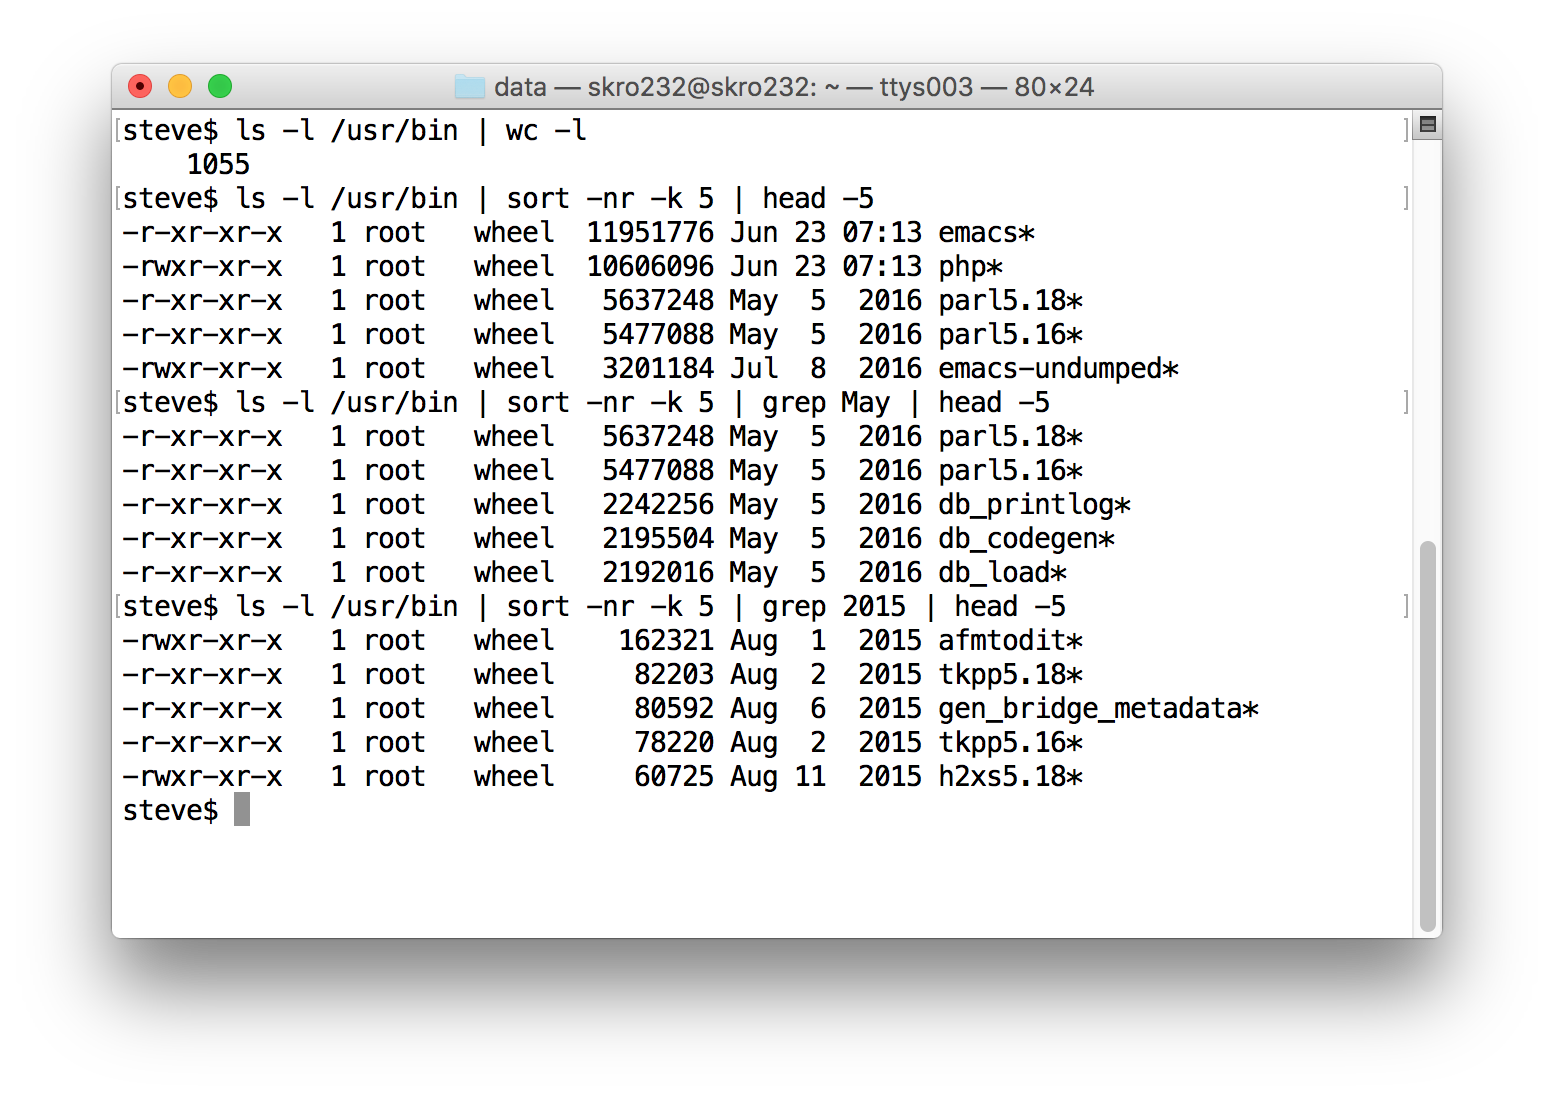
\includegraphics[width=10cm,scale=0.4]{images/pipes.png}
  \note{}
\end{frame}

\begin{frame}{What to type for a given command}
  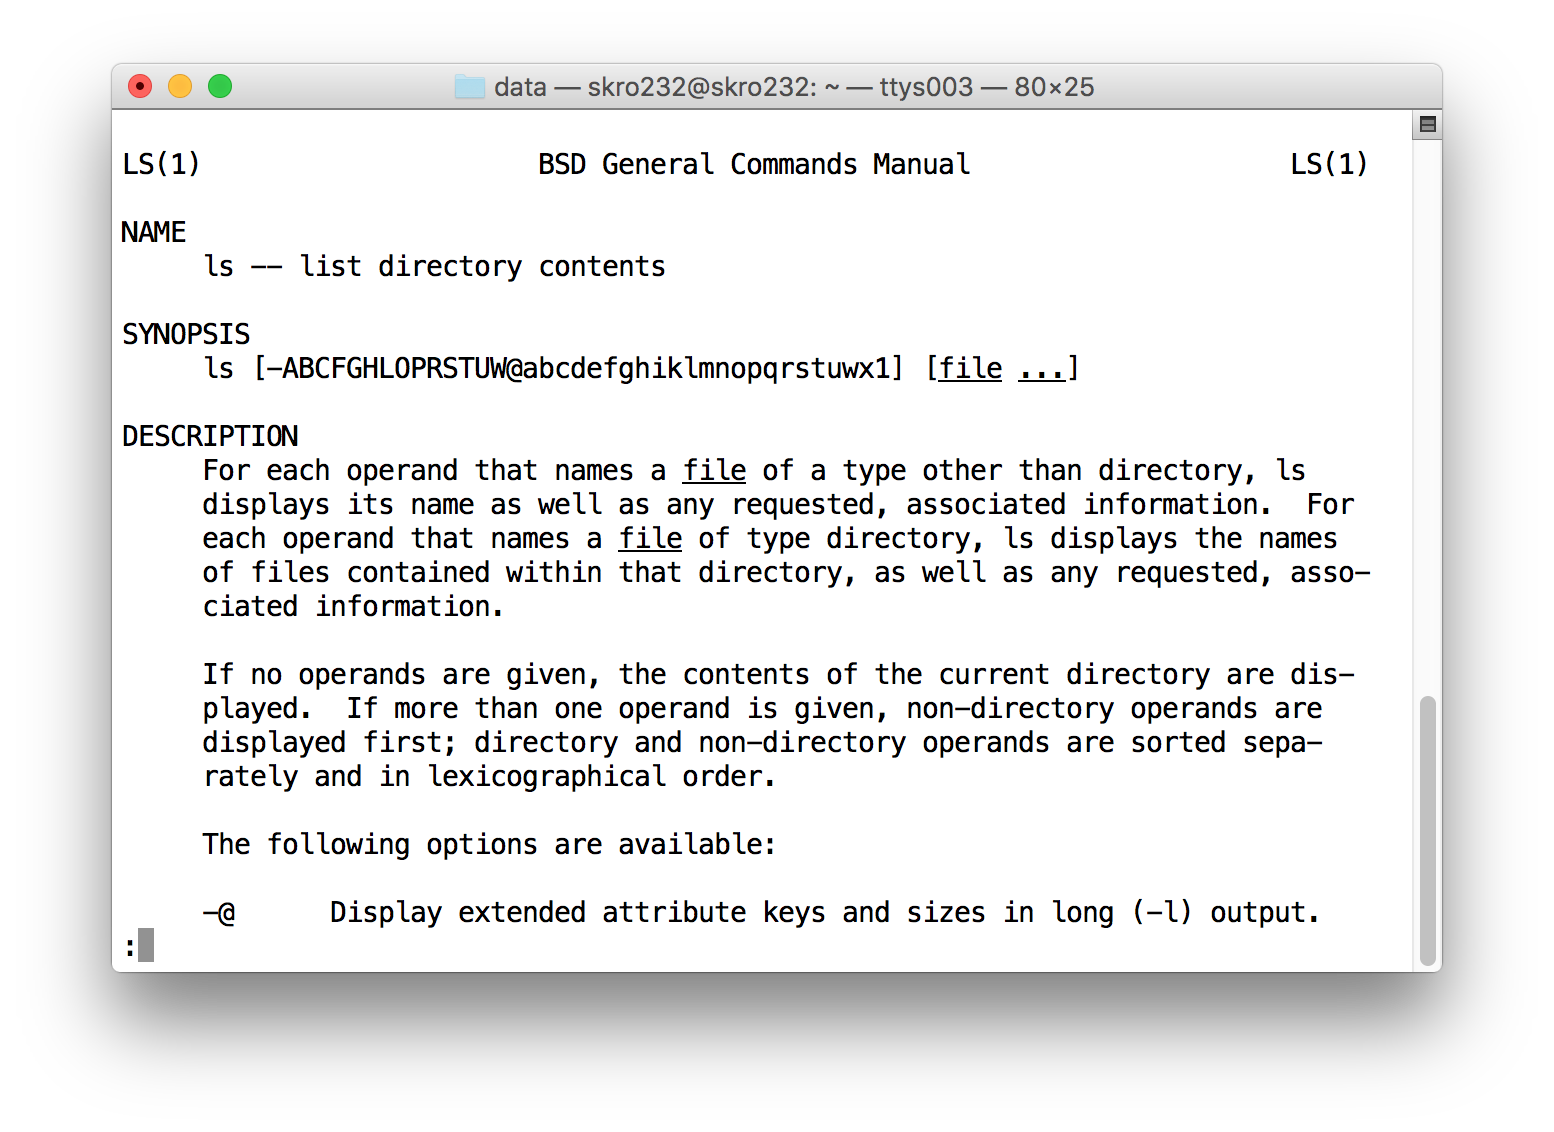
\includegraphics[width=10cm,scale=0.4]{images/manls.png}
  \begin{itemize}
  \item \texttt{man} \textit{command}  provides the manual page for \textit{command}
  \item  \texttt{man ls} in the example above
  \end{itemize}
  \note{}
\end{frame}

\begin{frame}{Man pages}
  \begin{itemize}
  \item \texttt{man} pages contain multiple sections
  \item Typical sections include:
    \begin{itemize}
    \item NAME - name of the command and brief discussion
    \item SYNOPSIS - how to invoke the command and list of arguments
    \item DESCRIPTION - detailed description of the program
    \item OPTIONS - options and their description
    \item EXAMPLES - example invocations and what they do
    \item EXIT STATUS - \texttt{exit(2)} codes (0 indicates success) 
    \item ENVIRONMENT - how shell variables affect program
    \item SEE ALSO - other programs or documents to consult
    \item BUGS - known issues
    \end{itemize}
  \end{itemize}
  \note{}
\end{frame}

\begin{frame}{Man pages - cont.}
  \begin{itemize}
  \item UNIX documentation system
  \item Organized into multiple sections
    \begin{itemize}
    \item 1 - programs or shell commands
    \item 2 - System (kernel) calls
    \item 3 - Library calls
    \item 4 - Special files (usually found in /dev)
    \item 5 - File formats
    \item 6 - Games
    \item 7 - Miscellaneous
    \item 8 - System administration commands (root)
    \item 9 - Non-standard kernel commands
    \end{itemize}
  \end{itemize}
  \note{}
\end{frame}

\begin{frame}{Man pages - How to find commands with 'man -k'}
  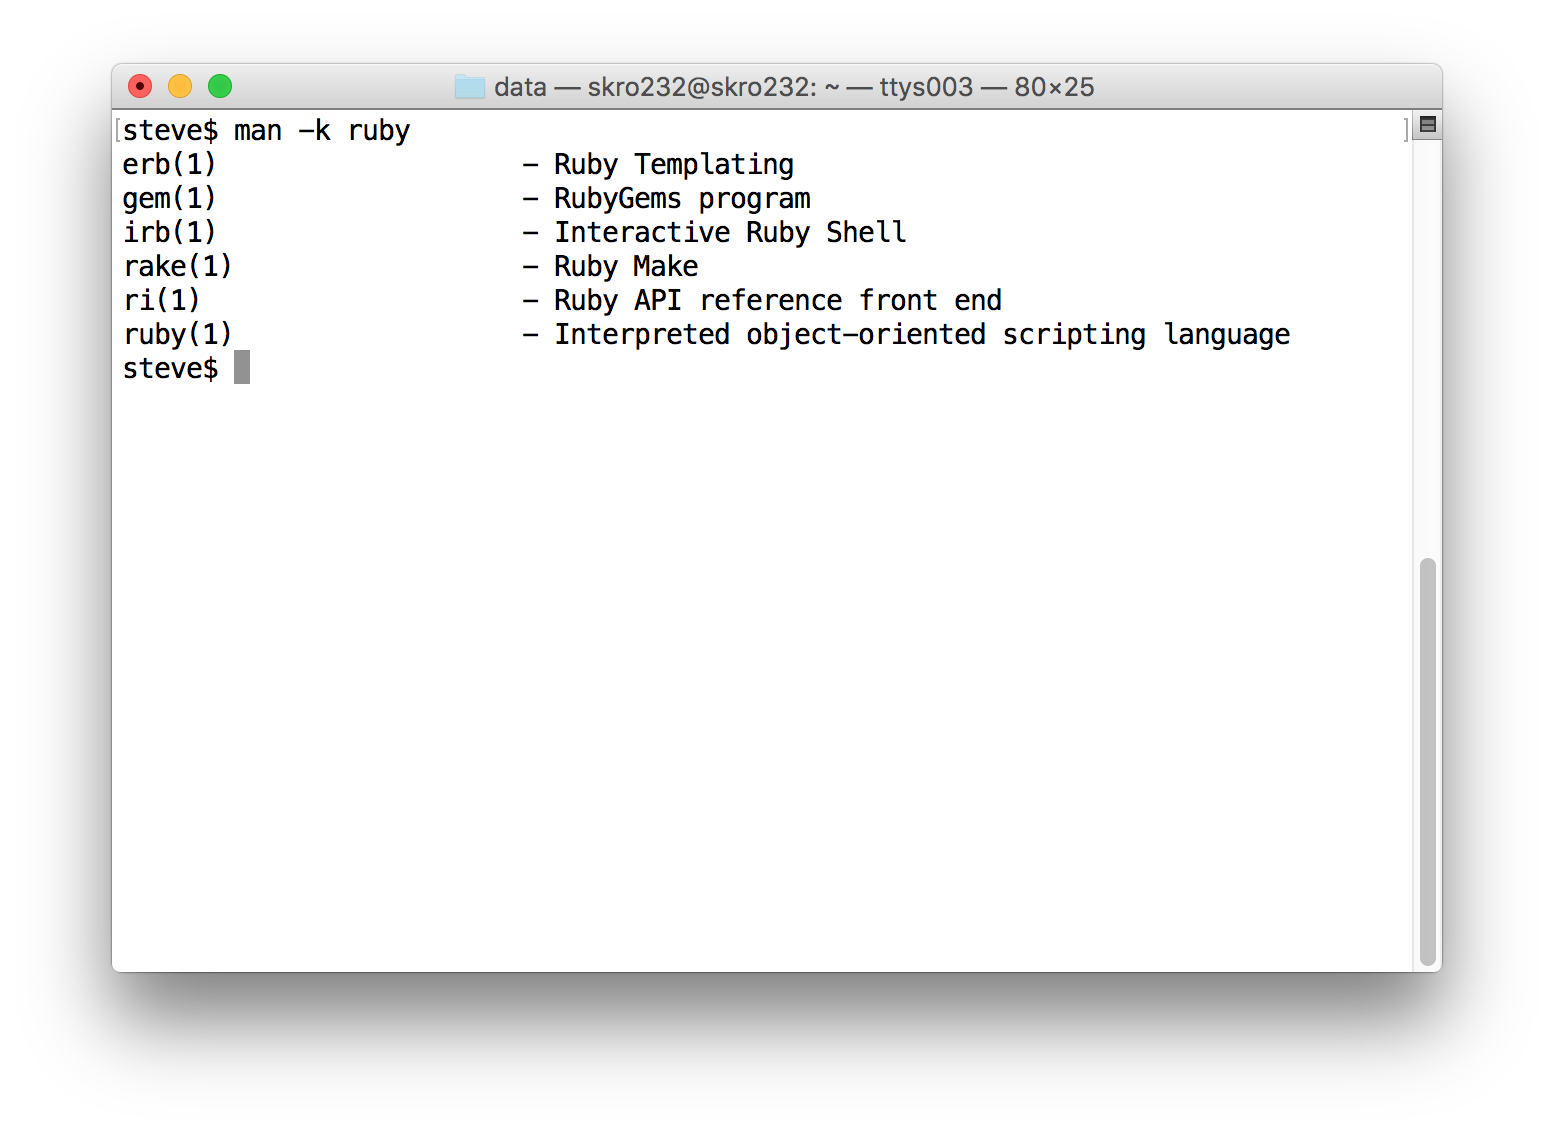
\includegraphics[width=10cm,scale=0.4]{images/man-k.png}
  \note{man -k 'ruby'}
\end{frame}

\begin{frame}{Regular expressions - searching text}
  \begin{itemize}
  \item Regular expressions allow you to search using string patterns
  \item Many programs in *NIX use regular expressions
  \item Most characters match themselves, 'abc' matches the
    string  ``abc''
  \item Meta characters:
    \begin{itemize}
    \item \texttt{\^{ }}  matches the beginning of a line
    \item \texttt{\$} matches the end of a line
    \item \texttt{.} matches a single character
    \item \texttt{?} matches zero or one of the preceding pattern
    \item \texttt{*} matches zero or more of the preceding pattern
    \item \texttt{+} matches zero or more of the preceding pattern
    \item \texttt{$\lbrack$} and \texttt{$\rbrack$} indicate the start and end of a character class
    \item \texttt{(} and \texttt{)} indicate the start and end of an atom
%    \item $\mid$ indicates an alternate
%    \item $\setminus$ before one of the above indicates an ordinary character
    \end{itemize}
  \item \texttt{$\setminus$} escapes meta characters: \texttt{$\setminus$\$} matches \texttt{\$}
  \end{itemize}
  
  \note{grep'}
\end{frame}

\begin{frame}{Regular expressions - examples}
  \begin{itemize}
  \item /abc/  matches ``abc''
  \item /[a-z]/ matches a lower case character
  \item /[a-z][A-Za-z0-9\_]+/ matches identifiers in many languages
  \item /\^{ }[0-9]+\$/ matches a line containing only a single integer
  \item /\^{ }a.*z\$/ matches a line starting with 'a' and ending with 'z'
  \end{itemize}
  \note{}
\end{frame}

\begin{frame}{Regular expressions - grep}
  \begin{itemize}
  \item \texttt{grep} (Global Regular Expression Print) is the standard search
    program
  \item \texttt{grep -i} PATTERN FILES - ignores case
  \item \texttt{grep -l} PATTERN FILES - prints just the FILES containing
    PATTERN
  \item \texttt{grep -f} RE\_FILE FILES - reads regular expressions, one per
    line, from RE\_FILE
  \end{itemize}
  \note{}
\end{frame}

\begin{frame}{\texttt{find} - Query your file system}
%%  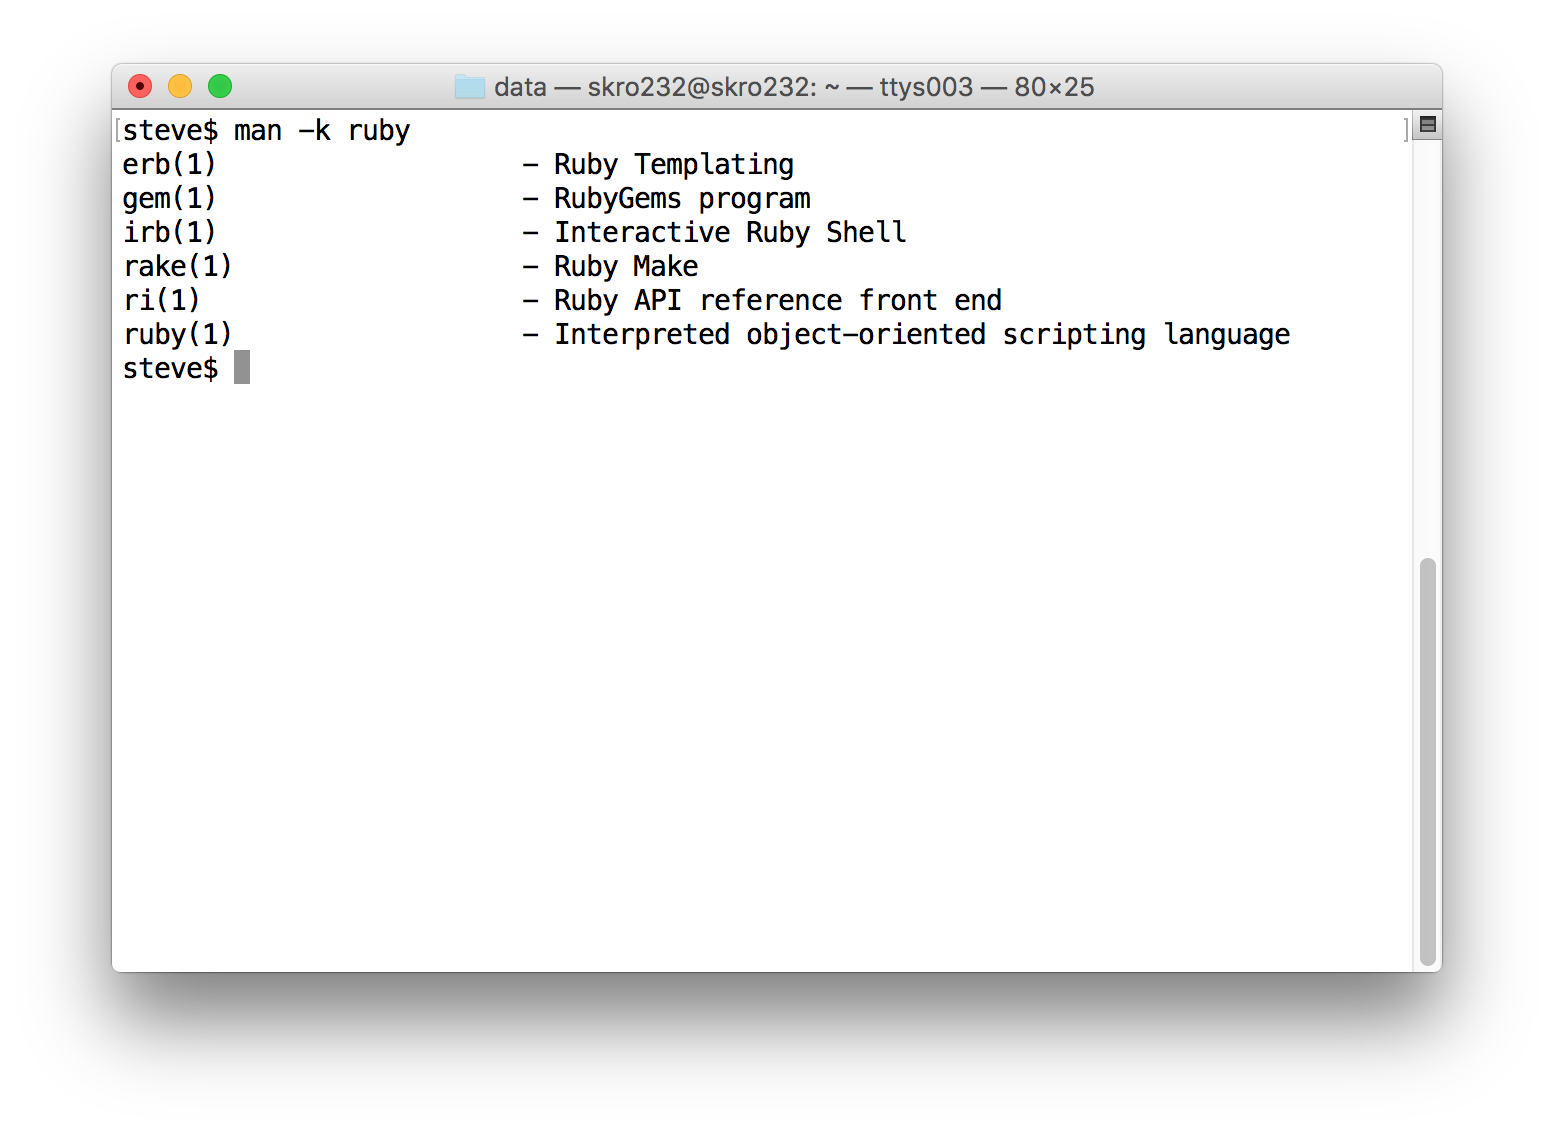
\includegraphics[width=10cm,scale=0.4]{images/man-k.png}
  \begin{itemize}
  \item \texttt{find} traverses a file system performing an action on each file it matches
  \item It provides many filters to fine tune a query:
    \begin{itemize}
    \item file name pattern
    \item file types (regular file, directories, links)
    \item file properties (create time, modification time, etc.)
    \item owner, group
    \item number of links
    \item and more
    \end{itemize}
  \item Default action is print the name of the file
  \end{itemize}
  \note{}
\end{frame}

\begin{frame}{\texttt{find} - Example}
  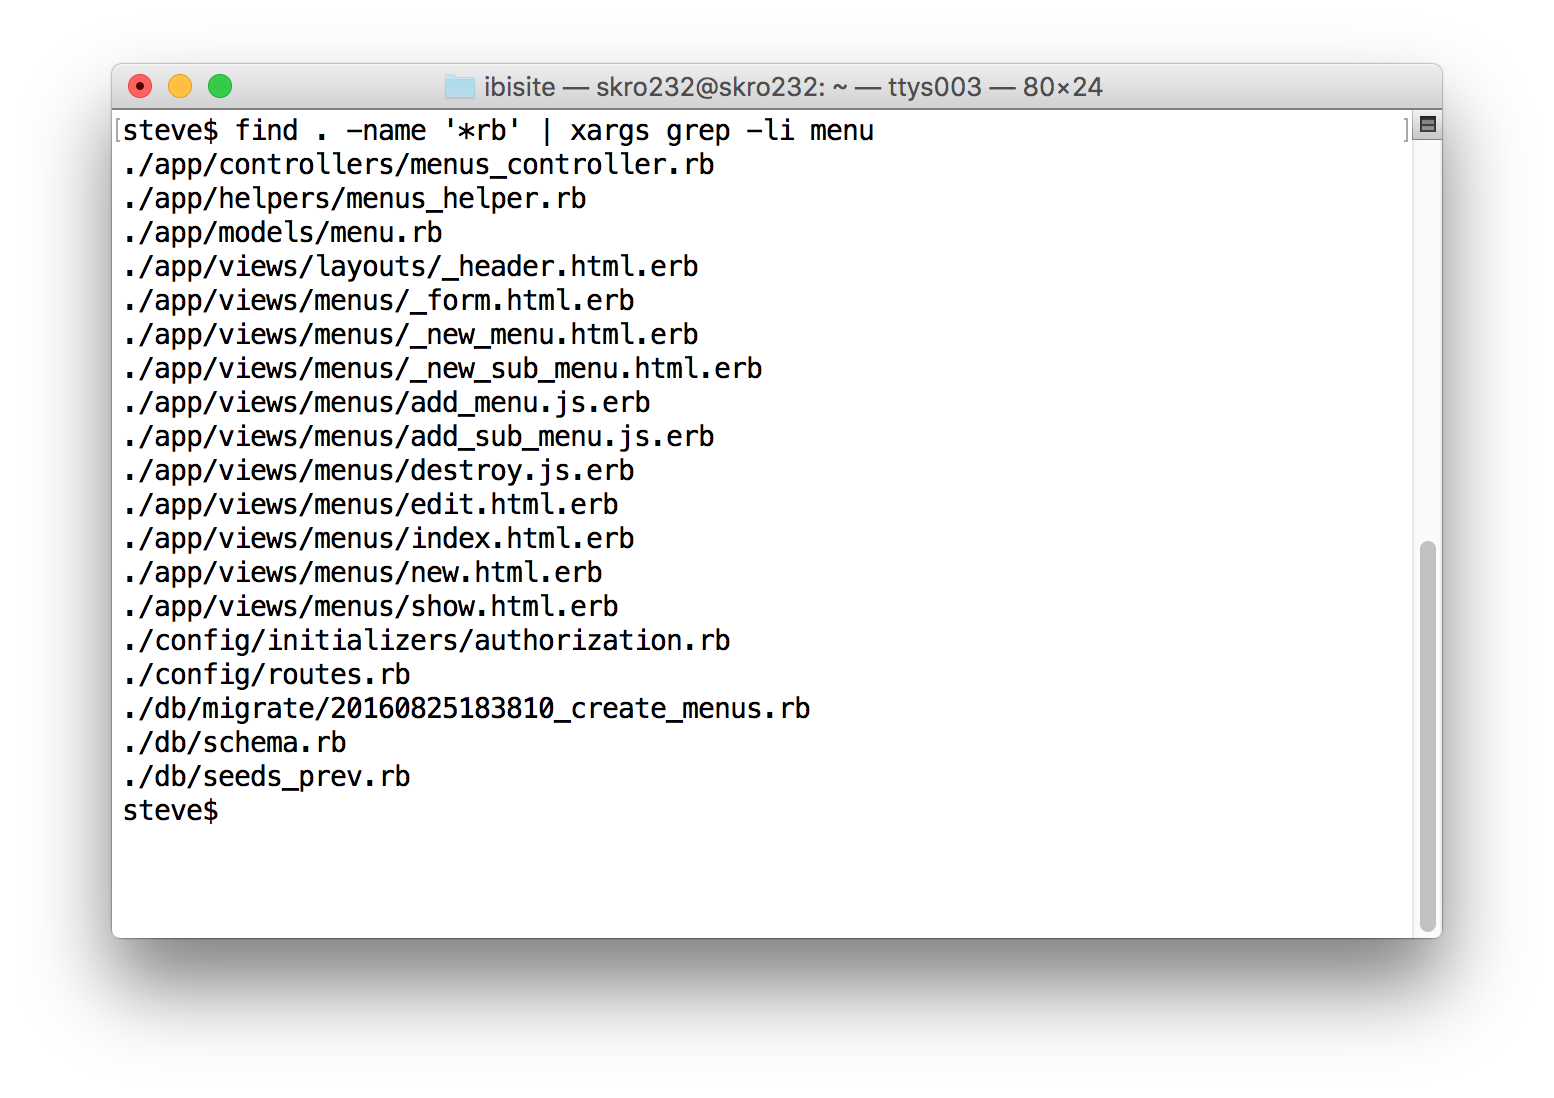
\includegraphics[width=10cm,scale=0.4]{images/find.png}
%%  \begin{itemize}
%%  \item 
%%  \end{itemize}
  \note{}
\end{frame}

\begin{frame}{\texttt{find} - Example using sed to filter}
  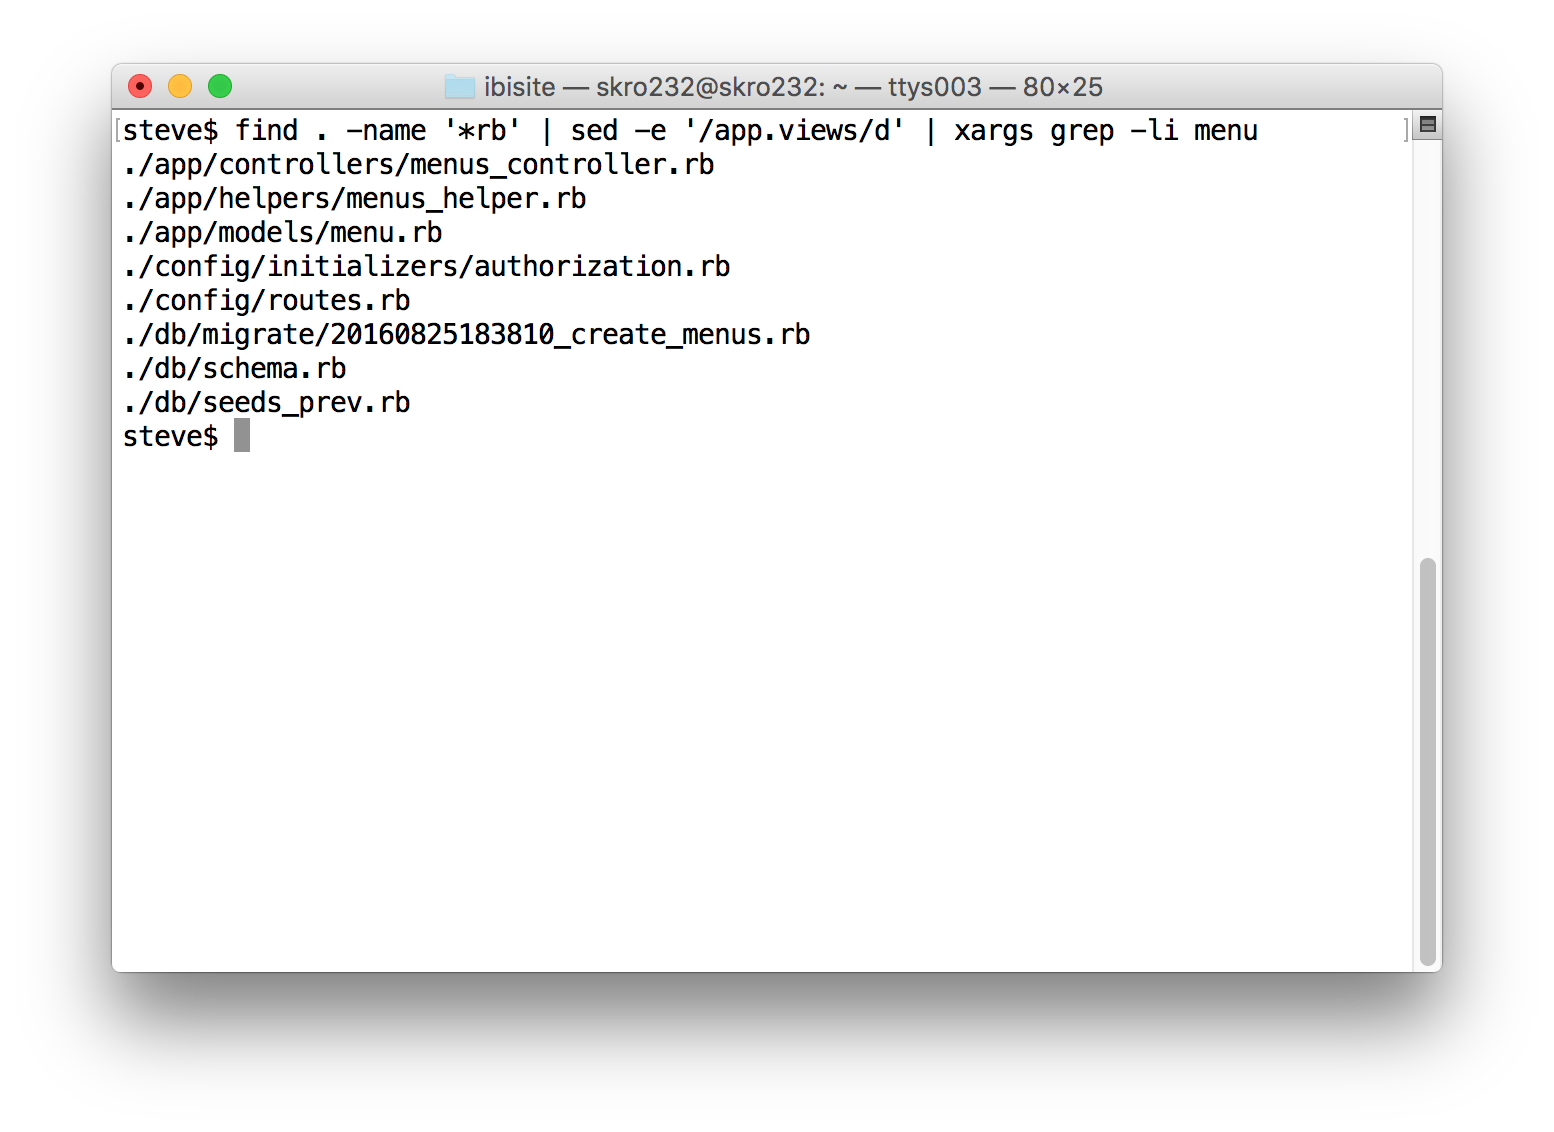
\includegraphics[width=10cm,scale=0.4]{images/find-1.png}
%%  \begin{itemize}
%%  \item 
%%  \end{itemize}
  \note{}
\end{frame}

\begin{frame}{Command substitution - use the shell to write your commands}
%%  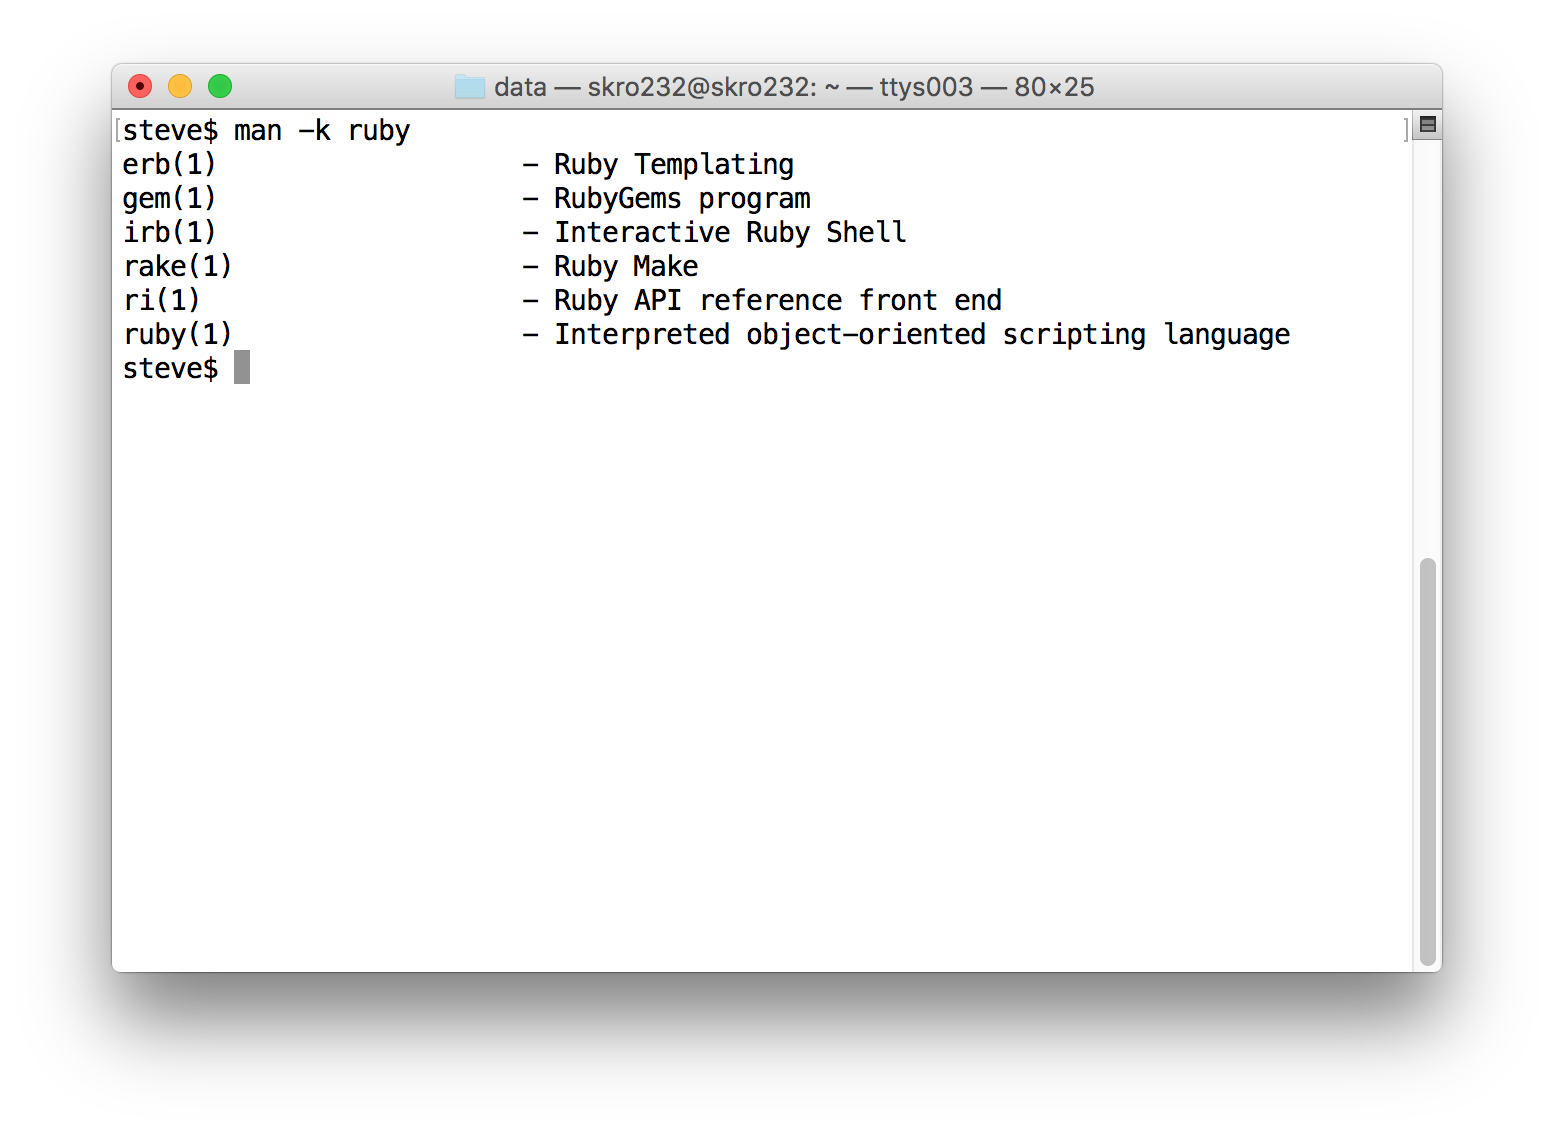
\includegraphics[width=10cm,scale=0.4]{images/man-k.png}
  \begin{itemize}
  \item \texttt{\$( \textit{pipe} ) } executes \textit{pipe} and
    substitutes the text in place
  \end{itemize}
  \note{}
\end{frame}

\begin{frame}{Command substitution - cont}
  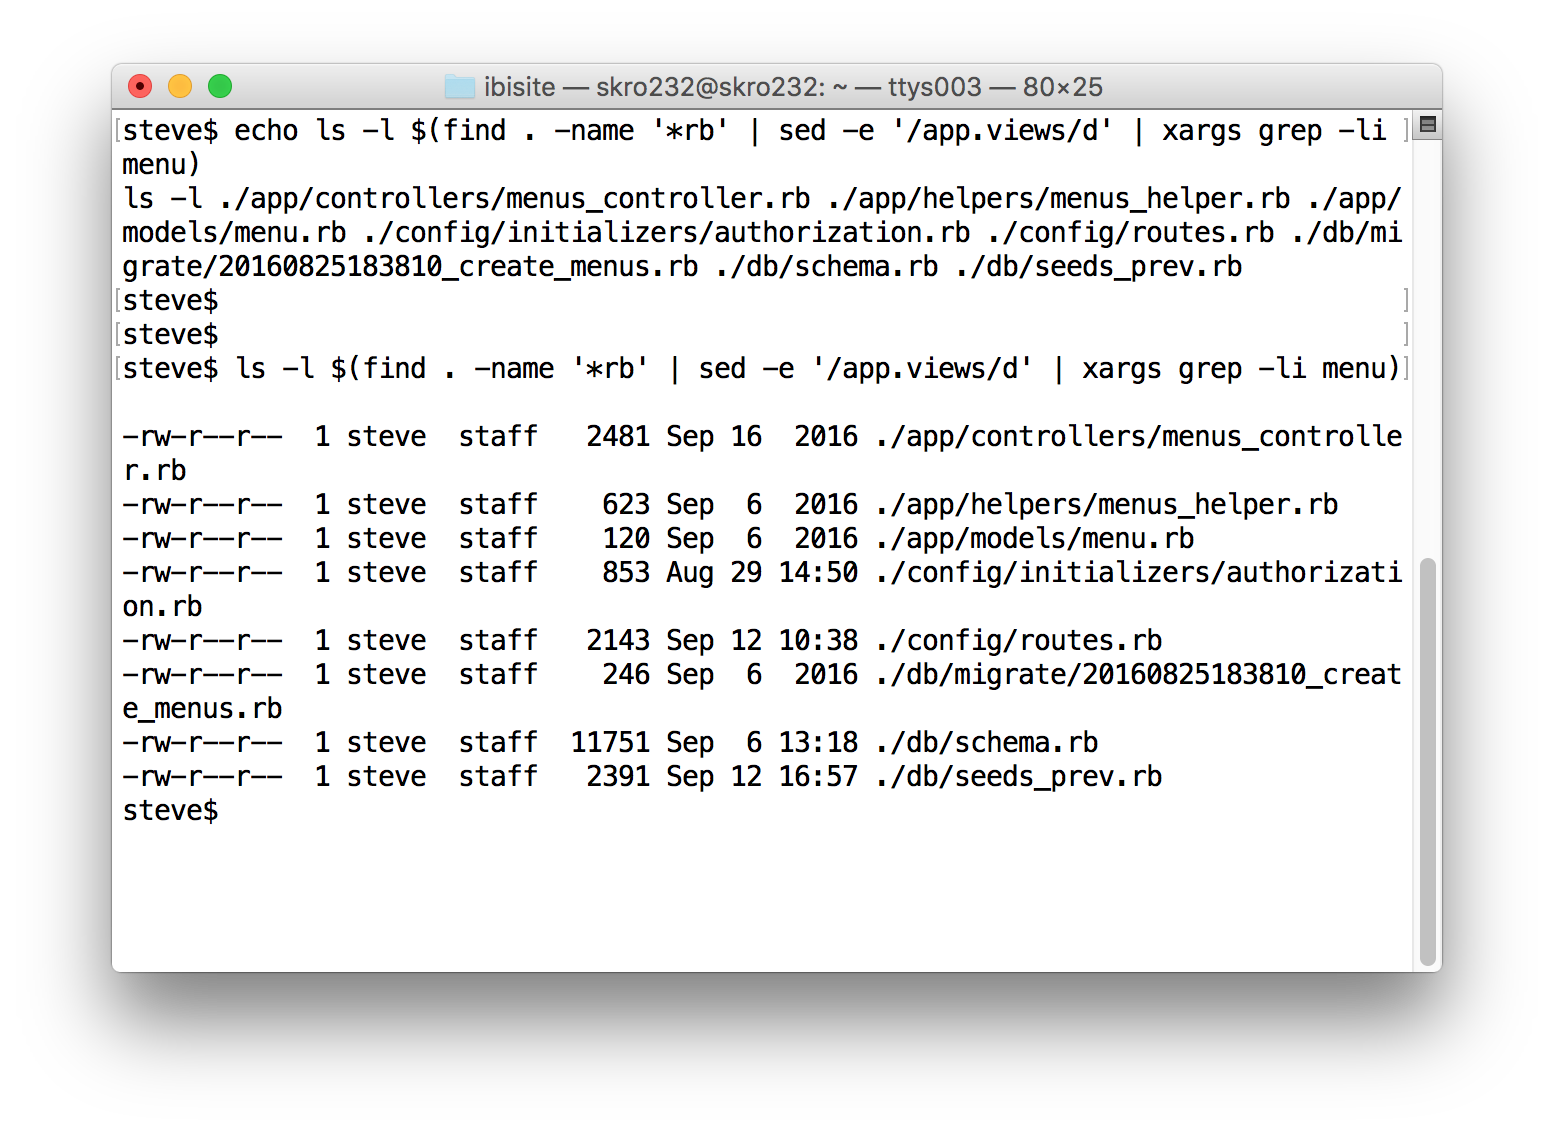
\includegraphics[width=10cm,scale=0.4]{images/cs-1.png}
%%  \begin{itemize}
%%  \item 
%%  \end{itemize}
  \note{}
\end{frame}

\begin{frame}{Command substitution - cont}
  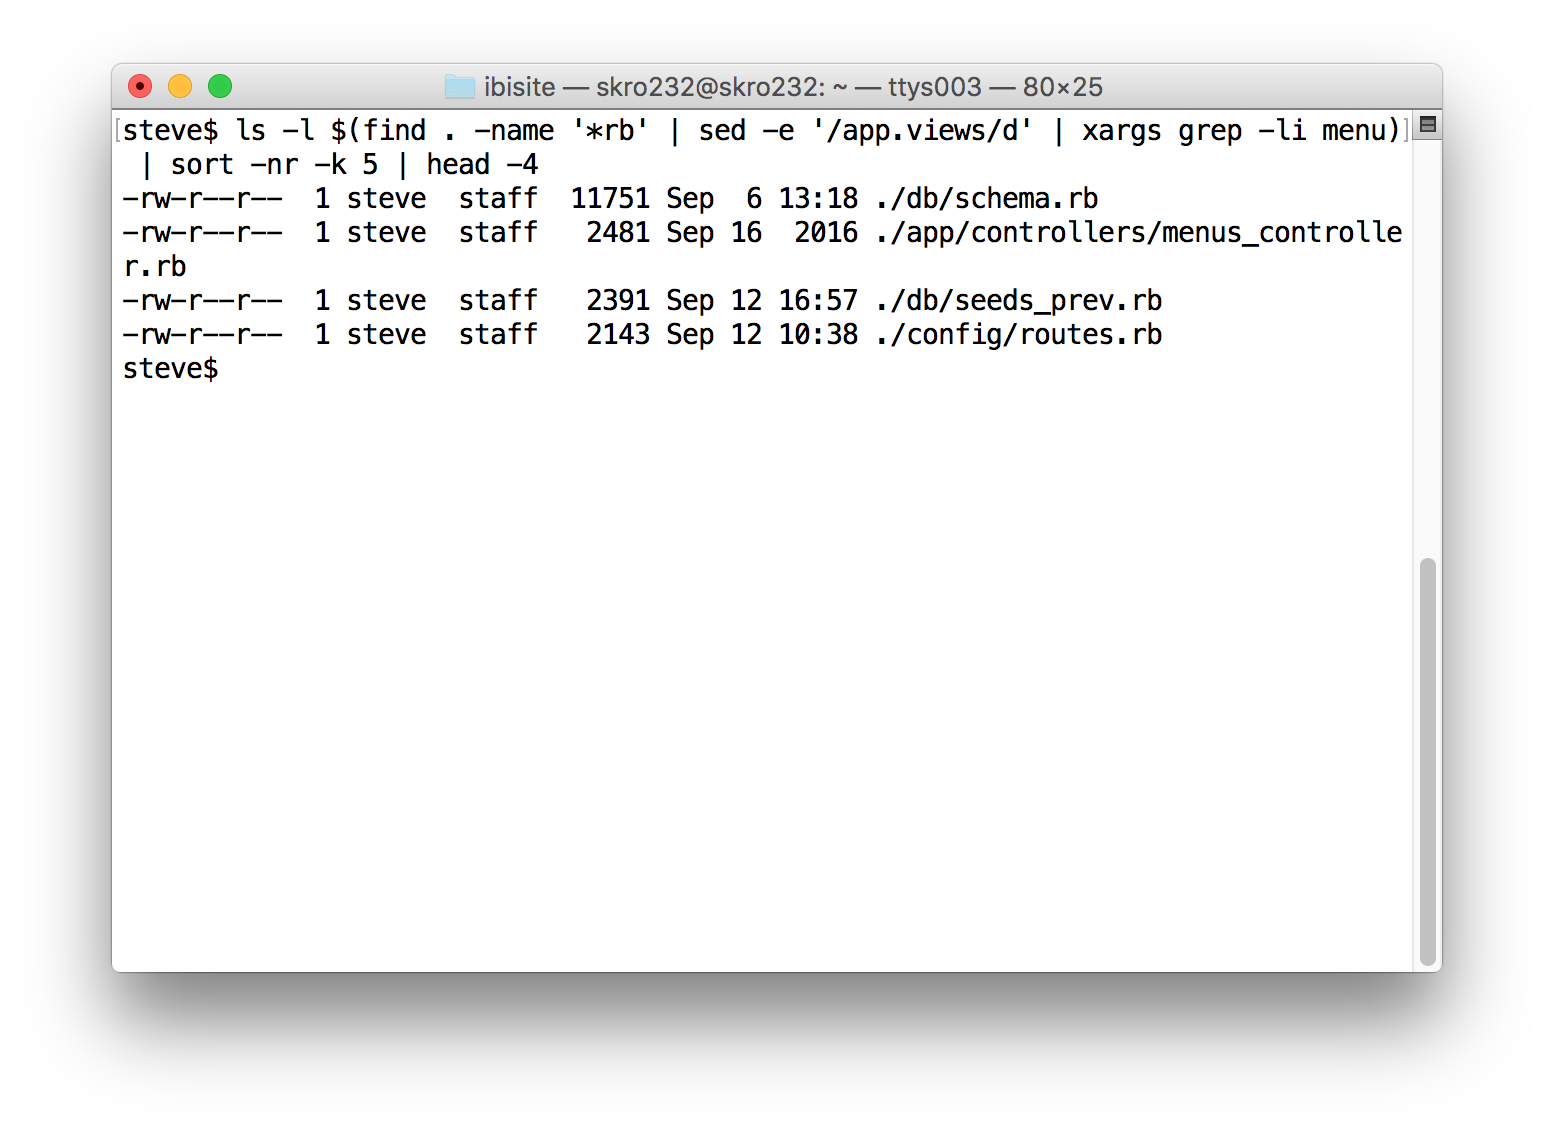
\includegraphics[width=10cm,scale=0.4]{images/cs-2.png}
%%  \begin{itemize}
%%  \item 
%%  \end{itemize}
  \note{}
\end{frame}

\begin{frame}{Common programs}
%%  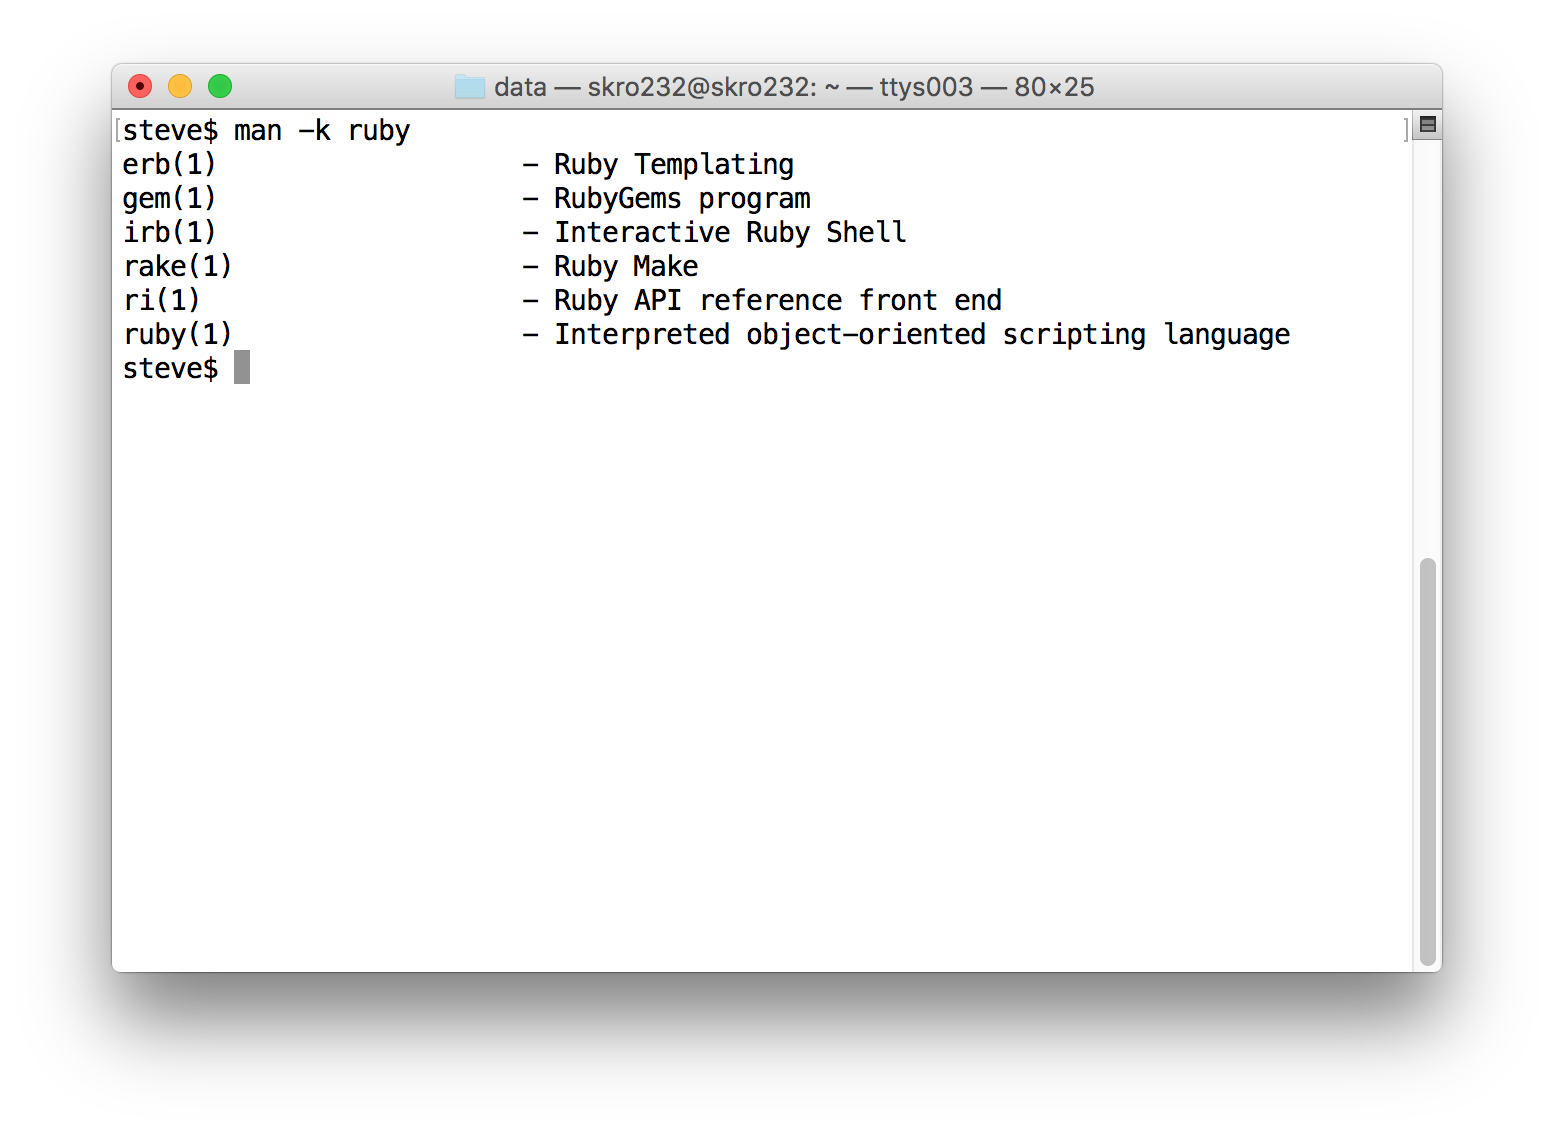
\includegraphics[width=10cm,scale=0.4]{images/man-k.png}
  \begin{itemize}
  \item \texttt{awk} - The AWK text processing language
    \pause
  \item \texttt{file} - describe the type of a file
    \pause
  \item \texttt{grep} - find strings in files
    \pause
  \item \texttt{less} - display a file a screen at a time
    \pause
  \item \texttt{ls} - list files
    \pause
  \item \texttt{sed} - Stream editor
    \pause
  \item \texttt{sort} - Sort lines of a file
    \pause
  \item \texttt{uniq} - Filters out repeated lines in sorted files
    \pause
  \item \texttt{wc} - Counts characters, words and lines of a file
    \pause
  \item \texttt{xargs} - used with \texttt{find} to execute a command on
    multiple files
  \end{itemize}
  \note{}
\end{frame}

\begin{frame}{Example problem - Solve NPR Sunday puzzle}
%%  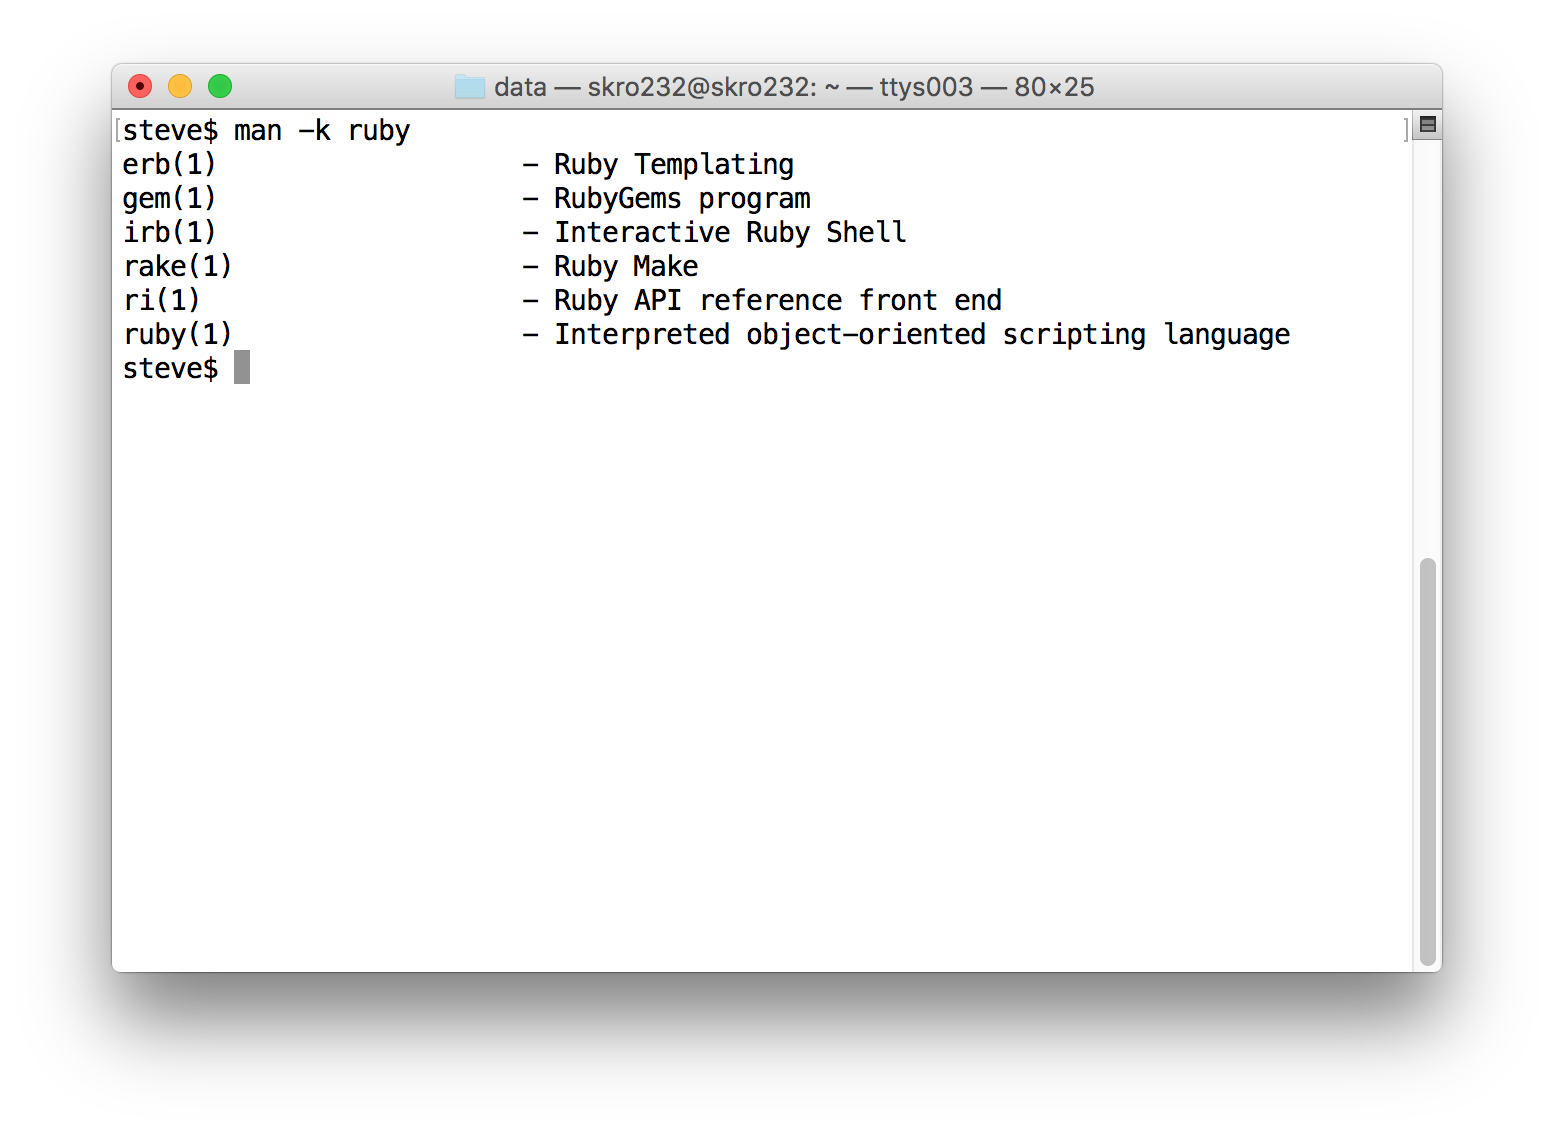
\includegraphics[width=10cm,scale=0.4]{images/man-k.png}

  From NPR Weekend Edition Sunday, Sept 4, 2016.

  \bigskip
  Next week's challenge, from listener Norm Baird of Toledo, Wash.: If
  you squish the small letters "r" and "n" too closely together, they
  look like an "m." Think of a common five-letter word with the
  consecutive letters "r" and "n" that becomes its own opposite if you
  change them to an "m."
  
  \bigskip
  About 840 people solved this puzzle.
  
  \bigskip
  Let's use our Ancient and Decrepit Tools to solve it in just two
  lines of code.
  \note{}
\end{frame}

\begin{frame}{}
  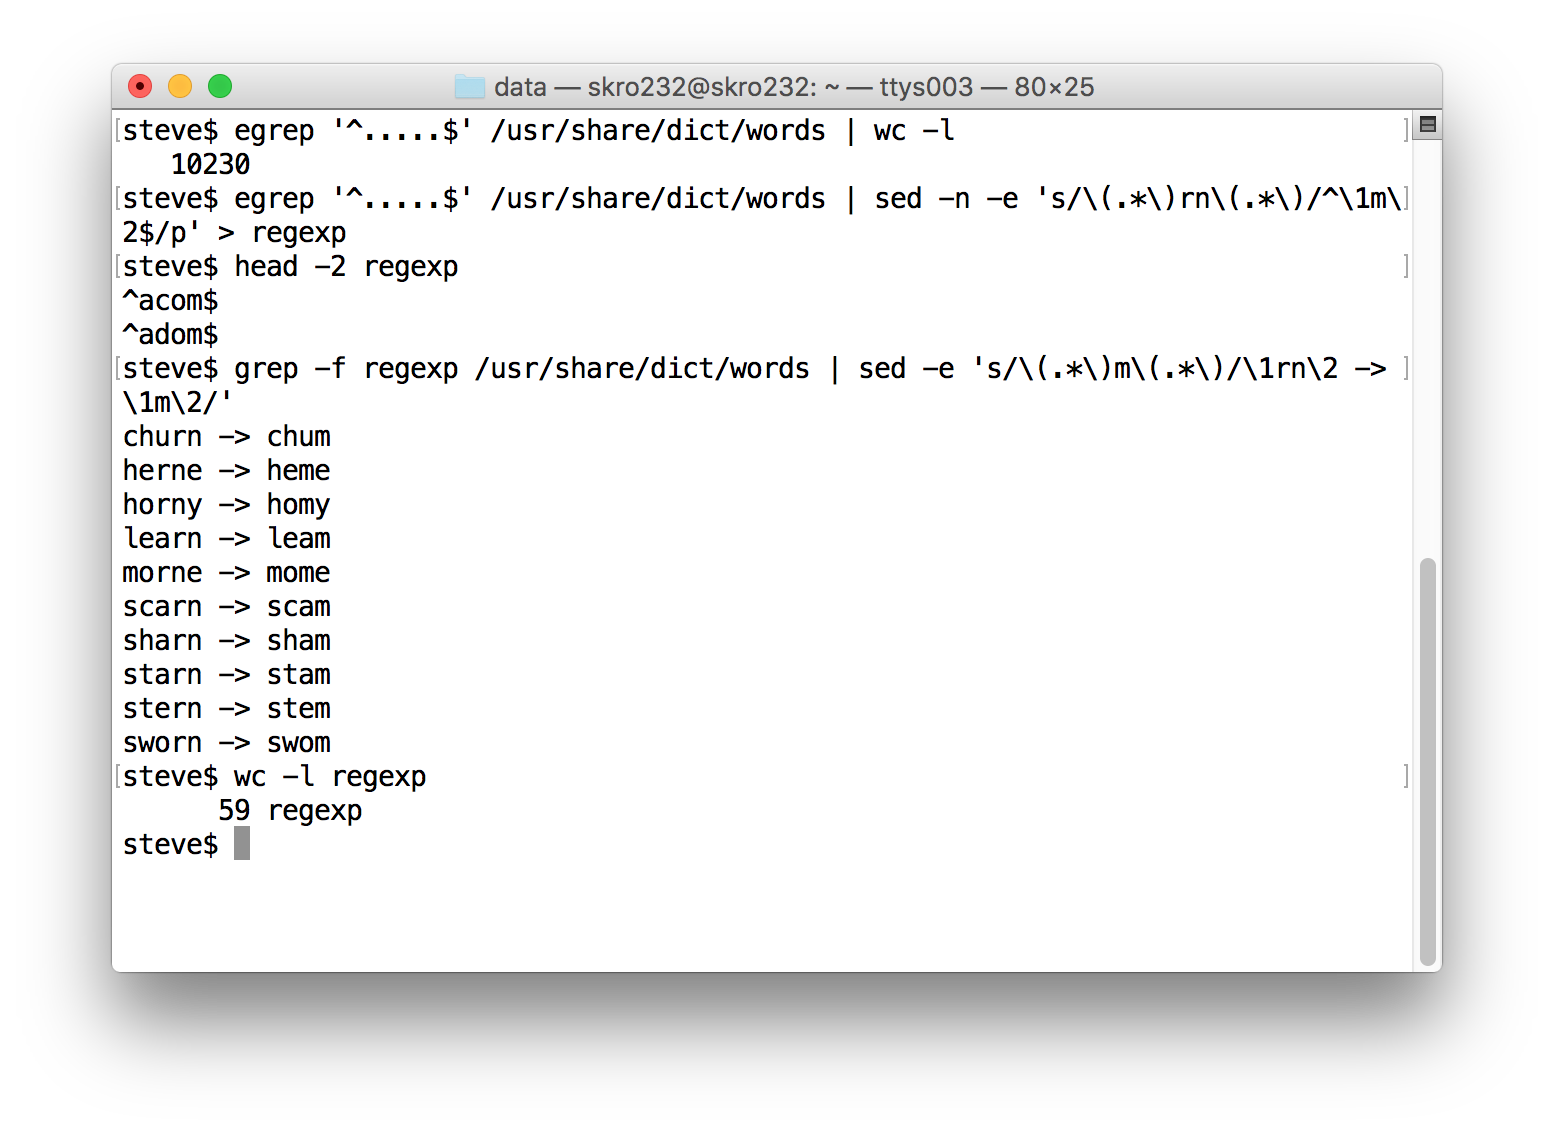
\includegraphics[width=10cm,scale=0.4]{images/puzzle.png}

  Answer: STERN and STEM
  \note{}
\end{frame}

\begin{frame}{Wrap up}
  \begin{itemize}
  \item Covered why you might want to use the command line
    \pause
  \item Described six concepts essential to efficient use of command
    line:
    \begin{itemize}
    \item Command shell
    \pause
    \item Pipes to connect commands
    \pause
    \item Man pages for documentation
    \pause
    \item Regular expressions for text processing
    \pause
    \item \texttt{find} to query file systems
    \pause
    \item Command substitution
    \end{itemize}
    \pause
  \item Demonstrated efficient command line use to solve an NPR Sunday puzzle
    in two lines of code
  \end{itemize}
  \note{}
\end{frame}

\begin{frame}{Questions?}
  \note{}
\end{frame}

\end{document}
